\chapter{Matrix Product States} \label{chap:MPS}
Numerical analysis of quantum many-body systems using exact diagonalization is highly limited by system size. Due to the large number of possible configurations in a many-body system and entanglement coupling various degrees of freedom, the Hilbert space grows too large for exact methods to search.
Consider the Bose-Hubbard model described in eq. \eqref{BHhamil}. The dimension of the corresponding Hilbert space is
\begin{equation}
	D_{\mathcal{H}} = \frac{(L+N_p -1)!}{N_p ! (L-1)!} \; ,
\end{equation}
where $L$ is the number of sites, and $N_p$ is the number of particles. For unit occupancy, $N_p / L = 1$, the Hilbert space grows exponentially with the system size \cite{Dong}. Therefore, descriptions using exact diagonalization are only possible for small systems.
Matrix product states parameterize the quantum states through a product of tensors, which can be depicted as a network. Decomposing the state as an explicitly contracted network of tensors enables efficient application of operators. Furthermore, the construction of matrix product states puts an upper bound on the entanglement entropy within the system, whereby states can be represented efficiently without considering unnecessary degrees of freedom \cite{Cramer}.\\
This chapter will cover the basics of matrix product states including their construction and freedom of gauges called canonical forms \cite{schollwock}. Furthermore, the generalization of MPS to operators called matrix product operators are introduced along with their applications. Algorithms involving matrix products states such as the DMRG method \cite{White1992,White1993} are introduced in the following chapter.


\section{Entanglement in Quantum Systems and Area Laws}
Entanglement is a fundamental property of quantum mechanics responsible for correlating different degrees of freedom within a quantum system. Thus, the individual parts of a quantum system can not be described alone, as entanglement with the remainder of the system has to be taken into consideration. This drastically complicates any description of the system, which is why exact descriptions of many-body systems are almost impossible.\\
The measure of entanglement within a quantum many-body system is the entanglement entropy, although it is often more instructive to look at the bipartite entanglement entropy, which measures the entanglement between two partitions of the system.
Consider a bipartition of the Hilbert space $\mathcal{H} = \mathcal{H}_A \otimes \mathcal{H}_B$. A state $\ket{\psi} \in \mathcal{H}$ can be decomposed using the \textit{Schmidt decomposition} as
\begin{equation}
	\ket{\psi} = \sum_{\alpha} \Lambda_{\alpha} \ket{\alpha}_A \otimes \ket{\alpha}_B \; ,
\end{equation}
where the states $\{ \ket{\alpha}_{A(B)} \}$ form an orthonormal basis of $\mathcal{H}_{A(B)}$, and $\Lambda_{\alpha} \ge 0$ are the Schmidt coefficients fulfilling $\sum_{\alpha} \Lambda_{\alpha}^2 = 1$ \cite{Pathak2013}. If only one term contributes to the Schmidt decomposition, the state is a product state i.e. the two parts of the Hilbert space are not mutually entangled. More terms implies that the state is entangled. From the Schmidt decomposition one can determine the reduced density matrix
\begin{equation}
	\rho_A = \Tr _B \ket{\psi}\bra{\psi} = \sum_{\alpha} \Lambda_{\alpha}^2 \ket{\alpha}_A \bra{\alpha}_A \; ,  
\end{equation}
by tracing out the subsystem $B$. 
From the Schmidt decomposition one can determine the entanglement entropy of the bipartition, which is defined as the von-Neumann entropy, $S$, of the reduced density matrix given by \cite{Pathak2013}
\begin{equation}
	S = - \sum_{\alpha} \Lambda_{\alpha}^2 \log \Lambda_{\alpha}^2 \; .
\end{equation}
Quite often, one is not concerned with the actual entanglement entropy of the system, but rather how it scales when the region in question grows in size. It is natural to assume that the entanglement entropy scales with  the \textit{volume} of the system, since this is the case for thermal systems. However, ground states of one-dimensional quantum many-body systems often follow an \textit{area law}, meaning that the scaling of the entropy is linear in the boundary area of the region. This is especially the case for systems with a gapped and local Hamiltonian \cite{Cramer}.\\
In a one dimensional lattice the boundary size of a bipartition is constant  independently of where the cut is made. Hence, the entanglement entropy will be bounded above, if the system follows an area law. This can be understood intuitively, as only degrees of freedom within the correlation length, $\xi$, of the boundary will be entangled, no matter where in the system the boundary is present \cite{Hastings2007}. This observation is the key to the success of numerical computations for one-dimensional systems, as the limited degree of entanglement enables the truncation of unused eigenstates without loss of accuracy in the representation of the state. Thus, many different states can be efficiently described by tensor networks despite existing in an exponentially large Hilbert space.


\section{Construction of an MPS} \label{sec:construct_MPS}
Matrix products states are parameterizations of one dimensional quantum states through a product of tensors. This parameterization is especially intuitive for lattice systems, as each lattice site can be represented by a single tensor. These tensors have two different kinds of indices; \textit{physical indices}, $j$, which corresponds to the local, physical states at a given site, and \textit{bond indices}, $\alpha$, which serves to connect neighbouring sites.
The dimension of the physical index is equal to that of the underlying Fock space, while the dimension of virtual bond index is related to the entanglement entropy between the two connected sites.
Tensors can be merged by contracting the bond connecting them, which is done by summing over their common index. Equations involving matrix product states tend to grow quite long, whereby they often are described through diagrams. In the diagrammatic representation the physical indices are marked by vertical legs, while bond indices are marked by horisontal legs. When two tensors are connected by a leg, it means that the corresponding bond is contracted. Further details and examples regarding tensor diagrams can be found in Appendix \ref{chap:diagrams}.

Consider a chain of $L$ sites with each site having a $d$-dimensional local Hilbert space $\{ \ket{j_n} \}$, where $n = 1, \ldots, L$. An arbitrary quantum state of this system reads
\begin{equation}
	\ket{\psi} = \sum_{j_1, \ldots, j_L} c_{j_1 \ldots j_L} \ket{j_1, \ldots, j_L} \; .
	\label{eq:arbstate}
\end{equation}
This description of a general state can be parametrized to the MPS form by applying successive Schmidt decomposition. However, in practice this is done through Singular Value Decompositions (SVD), as these are faster to perform numerically. The two approaches are equivalent, as the singular value decomposition is essentially a restatement of the Schmidt decomposition \cite{Pathak2013}.
Through an SVD, an arbitrary matrix, $A$, of dimensions $(M \times N)$ can be decomposed into three matrices, $A = U S V^{\dag}$, with the following properties \cite{schollwock}:
\begin{itemize}
\item
$U$ is of dimension $(M \times \min(M,N))$ and has orthonormal columns, meaning $U^{\dag}U = I$. If $M \leq N$, then it is also unitary $U U^{\dag} = I$.

\item
$S$ is a positive, diagonal $(\min(M,N) \times \min(M,N))$ matrix. The diagonal elements are singular values, and the number of non-zero entries is the Schmidt rank of $A$.

\item
$V^{\dag}$ is of dimension $(\min(M,N) \times N)$ and has orthonormal rows, meaning $V^{\dag}V = I$. If $M \geq N$, then it is also unitary $V V^{\dag} = I$.
\end{itemize} 
From the general state of eq. \eqref{eq:arbstate} an MPS can be constructed through the following steps:
\begin{enumerate}
\item
The $d^L$-dimensional vector $c_{j_1 \ldots j_L}$ is reshaped into a $(d \times d^{L-1})$ matrix $\Psi_{j_1 , (j_2 \ldots j_L)}$. Performing an SVD on $\Psi$ yields
\begin{equation}
	c_{j_1 \ldots j_L} = \Psi_{j_1 , (j_2 \ldots j_L)} = \sum_{\alpha_1}^{d} U_{j_1 , \alpha_1} S_{\alpha_1 , \alpha_1} (V^{\dag})_{\alpha_1 , (j_2 \ldots j_L)} = \sum_{\alpha_1}^{d} A_{\alpha_1}^{j_1} \Psi_{(\alpha_1 j_2),(j_3 \ldots j_L)} \; ,
\end{equation}
where $U$ has been reshaped into $d$ row vectors $A^{j_1}$ with entries $A_{\alpha_1}^{j_1} = U_{j_1 , \alpha_1}$. In this notation $A_{\alpha_1}^{j_1}$ is a tensor with physical indices $j_1$ and bond indices $\alpha_1$. Furthermore, $S$ and $V^{\dag}$ has been multiplied and reshaped into a $(d^2 \times d^{L-2})$ matrix, $\Psi_{(\alpha_1 j_2),(j_3 \ldots j_L)}$.

\item
The new matrix $\Psi_{(\alpha_1 j_2),(j_3 \ldots j_L)}$ is subjected to an SVD decomposition
\begin{equation}
	c_{j_1 \ldots j_L} = \sum_{\alpha_1}^{d} \sum_{\alpha_2}^{d^2} A_{\alpha_1}^{j_1} U_{(\alpha_1 j_2) , \alpha_2} S_{\alpha_2 , \alpha_2} (V^{\dag})_{\alpha_2 , (j_3 \ldots j_L)} = \sum_{\alpha_1}^{d} \sum_{\alpha_2}^{d^2} A_{\alpha_1}^{j_1} A_{\alpha_1 , \alpha_2}^{j_2} \Psi_{(\alpha_2 j_3),(j_4 \ldots j_L)} \; ,
\end{equation}
where $U$ has been decomposed into $d$ matrices $A^{j_2}$ with entries $A_{\alpha_1 , \alpha_2}^{j_2} = U_{(\alpha_1 j_2) , \alpha_2}$. The matrix $\Psi_{(\alpha_2 j_3),(j_4 \ldots j_L)}$ has dimensions $(d^3 \times d^{L-3})$ and is yet again a product of the matrices $S$ and $V^{\dag}$ from the SVD.

\item
The procedure detailed in the two previous steps is continued throughout the chain leaving 
\begin{equation}
	c_{j_1 \ldots j_L} = \sum_{\alpha_1 , \ldots , \alpha_{L-1}} A_{\alpha_1}^{j_1} A_{\alpha_1 , \alpha_2}^{j_2} \ldots A_{\alpha_{L-2} ,\alpha_{L-1}}^{j_{L-1}} A_{\alpha_{L-1} ,\alpha_{L}}^{j_{L}} \equiv A^{j_1} A^{j_2} \ldots A^{j_{L-1}} A^{j_{L}} \; ,
\end{equation}
where the sum can be recognized as a matrix multiplication allowing a neater notation.
\end{enumerate}
\begin{figure}[h!]
	\centering
	\begin{tikzpicture}[inner sep=1mm]
	\def \numb {7};
	\def \hdist {1.5};
	\def \wid {10};
	\def \wids {8.5};

	\node[tensor, minimum width=\wid cm] (tens1) at (\wid/2 +1, 0) {$c^{j_1 \ldots j_N}$};
	
	\foreach \i in  {1,...,\numb} {
		\node (\i) at (\i*\hdist, -0.8) {};
		\draw[-] (\i) -- (\i |-  tens1.south);	
	};
	
	\draw[->, line width=1.25mm] (\wid/2 +1,-1) -- (\wid/2 +1,-2.3);
	
	\node[tensorl] (blok1) at (1*\hdist, -3) {$A^{j_1}$};
	\node[tensor, minimum width=\wids cm] (tens2) at (\wids/2 +2.5, -3) {$c^{j_2 \ldots j_N}$};
	
	\foreach \i in  {2,...,\numb} {
		\node (\i) at (\i*\hdist, -3.8) {};
		\draw[-] (\i) -- (\i |-  tens2.south);	
	};
	\node (node1) at (1*\hdist, -3.8) {};
	\draw[-] (node1) -- (blok1);
	\draw[-] (tens2) -- (blok1);
	
	\node (dots) at (\wid/2 +1, -4.6) {\vdots};
	
	\foreach \i in  {1,...,\numb} {
		\node[tensorl] (t\i) at (\i*\hdist, -6) {};
		\node (\i) at (\i*\hdist, -6.8) {};
		\draw[-] (t\i) -- (\i);	
	};
	\foreach \i in  {1,...,6} {
		\pgfmathtruncatemacro{\iplusone}{\i + 1};
		\draw[-] (t\i) -- (t\iplusone);	
	};
	
	\node[tensorl] (lab1) at (1*\hdist, -6) {$A^{j_1}$};
	\node[tensorl] (lab2) at (2*\hdist, -6) {$A^{j_2}$};
	\node[tensorl] (labN) at (\numb*\hdist, -6) {$A^{j_N}$};
	
\end{tikzpicture}
	\caption{\textit{Diagrammatic representation of the construction of a left-canonical MPS from an arbitrary quantum state through successive SVD's.}}
	\label{fig:MPSbuild}
\end{figure}
The construction of an MPS is illustrated in figure \ref{fig:MPSbuild}. Thereby, the original state (equation \ref{eq:arbstate}) can be written as a matrix product state in the form \cite{schollwock}
\begin{equation}
	\ket{\psi} = \sum_{j_1, \ldots, j_L} A^{j_1} A^{j_2} \ldots A^{j_{L-1}} A^{j_{L}} \ket{j_1, \ldots, j_L} \; .
	\label{eq:MPS_LC} 
\end{equation}
Following the construction sequence, the dimensions of the matrices $A^{j_n}$ follow a pyramid-like structure $(1 \times d ),(d \times d^2) , \ldots , (d^{L/2 -1} \times d^{L/2}) , (d^{L/2} \times d^{L/2 -1 }), \ldots , (d \times 1)$, where $L$ is taken as even for simplicity. 
However, the state can be represented much more efficiently by truncating the dimensions of the matrices (bonds), due to the area law scaling of entanglement entropy \cite{EntropyScaling}. A bond dimension $\chi$ infers an entanglement entropy bounded by $S(\rho_A) = \mathcal{O}(\log \chi)$ \cite{Gillman2018}, whereby one often can discard the contribution of many eigenstates without loss of accuracy.

In practice this is done by keeping only the $D$ largest singular values of the SVD matrix $S$, as these contribute the most to the state. Alternatively  one can discard all eigenstates contributing with eigenvalues less than some threshold $\epsilon_t$.


\section{Canonical Forms}
\label{sec:canonical}
The MPS described in equation \ref{eq:MPS_LC} is not unique, as writing 
\begin{equation}
	\tilde{A}^{j_n} = X_{n-1} A^{j_n} X_{n}^{-1}
\end{equation}
describes the same state using different matrices. This gauge freedom allows expressing the MPS in whichever way is most convenient, which can greatly reduce the effort of applying operators and calculating overlaps. By choosing a gauge, the MPS is brought into a \textit{canonical form} \cite{Vidal2007}. The following examples detail bringing MPSs into canonical forms through construction, however, the same can be achieved for an already built MPS through successive SVDs and regrouping of the resulting matrices. 

\subsection{Left-canonical matrix product state}
The process of constructing an matrix product state detailed in Section \ref{sec:construct_MPS} brings the MPS in a \textit{left-canonical} form. This implies that all the matrices are left-normalized, such that
\begin{equation}
	\sum_{j_n} A^{j_n \dag} A^{j_n} = I \; .
	\label{eq:LC_ident}
\end{equation}
The left-normalization is a consequence of the matrix $U$ (from the SVD) fulfilling $U^{\dag}U = I$. Since the matrices $A^{j_n}$ are reshaped from $U$, these properties persists
\begin{align*}
	\delta_{\alpha_n , \alpha_n'} &= \sum_{\alpha_{n-1} j_n} (U^{\dag})_{\alpha_n , (\alpha_{n-1} j_n)} U_{(\alpha_{n-1} j_n), \alpha_n'} \\
	 &= \sum_{\alpha_{n-1} j_n} (A^{j_n \dag})_{\alpha_n , \alpha_{n-1}} A_{\alpha_{n-1}, \alpha_n'}^{j_n} \\
	 &= \sum_{j_n} \left( A^{j_n \dag} A^{j_n} \right)_{\alpha_{n} . \alpha_n'}
\end{align*} 
\begin{figure}[h!]
	\centering
	\begin{tikzpicture}[inner sep=1mm]
	\def \vdist {1.5};

	\node[tensorl] (tens1) at (1,0) {};
	\node[tensorl] (tens2) at (1,-\vdist) {}; 
 	
	\node (index1) at (2.5,0) {$\alpha_n$};
	\node (index2) at (2.5,-\vdist) {$\alpha_n '$}; 	
 	
 	\draw[-] (tens1) -- (tens2);
	\draw[-] (tens1) -- (index1);
	\draw[-] (tens2) -- (index2); 	
    \draw[-] (tens1.west) .. controls (0, 0) and (0, -\vdist) .. (tens2.west);
    
    
    \node (eq) at (3.5,-\vdist/2) {$=$};
    
    
 	\node (dummy1) at (5,0) {$\alpha_n$};
 	\node (dummy2) at (5,-\vdist) {$\alpha_n '$};
    
    \draw[-] (dummy1.west) .. controls (4, 0) and (4, -\vdist) .. (dummy2.west);
    
    \node (equiv) at (6.5,-\vdist/2) {$\equiv \quad \delta_{\alpha_n , \alpha_n '}$};
\end{tikzpicture}
	\caption{\textit{Contraction over the left index (shown as the arc) and the physical index of two left-normalised matrices. The result is $\delta_{\alpha_n , \alpha_n'}$, adding the n'th site to the contraction of all previous sites to the left.}}
	\label{fig:leftNorm}
\end{figure}
Figure \ref{fig:leftNorm} illustrates a contraction of the bonds connecting two left-normalised matrices. As this contraction results in the identity per definition, one can contract left-normalised matrices without any explicit calculation. The explicit contraction is displayed diagrammatically through an arc, which is equivalent to an identity-tensor with two bond indices. 


\subsection{Right-canonical matrix product state}
One could also have built a a right-canonical MPS from eq. \eqref{eq:arbstate}, had one performed the SVDs from other side of the chain. Constructing the MPS from the right implies multiplying $U$ and $S$ into the new $\Psi$-matrix, and reshaping $(V^{\dag})_{(\alpha_{n-1} j_n), \alpha_n}$ into matrices $B_{\alpha_{n-1} , \alpha_n}^{j_n}$. Hence, the right-canonical form of the MPS of eq. \eqref{eq:MPS_LC} reads
\begin{equation}
	\ket{\psi} = \sum_{j_1, \ldots, j_L} B^{j_1} B^{j_2} \ldots B^{j_{L-1}} B^{j_{L}} \ket{j_1, \ldots, j_L} \; .
\label{eq:MPS_RC}	 
\end{equation}
In this form all the matrices are right-normalized, whereby 
\begin{equation}
	\sum_{j_n} B^{j_n} B^{j_n \dag} = I \; .
	\label{eq:RC_ident}
\end{equation}
Note the reverse ordering of the matrix product compared to the left-normalized case. Figure \ref{fig:rightNorm} illustrates two right-normalised matrices contracted over their physical index.
\begin{figure}[h!]
	\centering
	\begin{tikzpicture}[inner sep=1mm]
	\def \vdist {1.5};
	
	\node[tensorr] (tens1) at (2.5,0) {};
	\node[tensorr] (tens2) at (2.5,-\vdist) {}; 
 	
	\node (index1) at (1,0) {$\alpha_n$};
	\node (index2) at (1,-\vdist) {$\alpha_n '$}; 	
 	
 	\draw[-] (tens1) -- (tens2);
	\draw[-] (tens1) -- (index1);
	\draw[-] (tens2) -- (index2); 	
    \draw[-] (tens1.east) .. controls (3.5, 0) and (3.5, -\vdist) .. (tens2.east);
    
    
    \node (eq) at (4,-\vdist/2) {$=$};
    
    
 	\node (dummy1) at (5,0) {$\alpha_n$};
 	\node (dummy2) at (5,-\vdist) {$\alpha_n '$};
    
    \draw[-] (dummy1.east) .. controls (6, 0) and (6, -\vdist) .. (dummy2.east);
    
    \node (equiv) at (7.5,-\vdist/2) {$\equiv \quad \delta_{\alpha_n , \alpha_n '}$};
\end{tikzpicture}
	\caption{\textit{Contraction over the right index (shown as the arc) and the physical index of two right-normalised matrices.}}
	\label{fig:rightNorm}
\end{figure}


\subsection{Mixed-canonical matrix product state}
In practice one rarely finds use for a purely left- or right-canonical MPS. However, combining the two canonical forms listed above yields the mixed-canonical form. The mixed-canonical results in a natural bi-partitioning of the system into a Schmidt decomposition, and it is especially useful for measuring local properties of the state \cite{schollwock}.\\
Consider the procedure of building an MPS in the left-canonical form, where $c_{j_1 \ldots j_L}$ has been decomposed from the left up until site $n$
\begin{equation}
	c_{j_1 \ldots j_L} = \sum_{\alpha_n} \left( A^{j_1} \ldots  A^{j_n} \right) _{\alpha_n} S_{\alpha_n , \alpha_n} (V^{\dag})_{\alpha_n , (j_{n+1} \ldots j_L)} \; .
\end{equation}
By reshaping $V^{\dag}$  into the matrix $\Psi_{(\alpha_n j_{n+1} \ldots j_{N-1}),j_N}$, one can initiate a successive decomposition from the right, resulting in a set of right-normalized matrices. The final result reads
\begin{equation}
	c_{j_1 \ldots j_N} = A^{j_1} \ldots A^{j_n} S B^{j_{n+1}} \ldots B^{j_L} \; ,
	\label{eq:mixedCanon}
\end{equation}
which is illustrated in figure \ref{fig:MixedCanonical1}.
\begin{figure}[h!]
\centering % <-- add this
\begin{subfigure}[b]{0.47\textwidth}
	\caption{}  	
  	\begin{tikzpicture}[inner sep=1mm]
	\def \hdist {1.5};
	\def \numb {5};
	\def \vleg {1};
	\def \NL {3};
	
	\node[minimum height=0.5 cm] (frame) at (1 ,0.5) {};

	\foreach \i in  {1,...,\NL} {
		\node[tensorl] (\i) at (\i*\hdist, 0) {};
		\node (index\i) at (\i*\hdist, -\vleg) {};
		\draw[-] (\i) -- (index\i);	
	};
	
	\foreach \i in  {1,...,2} {
		\pgfmathtruncatemacro{\iplusone}{\i + 1};
		\draw[-] (\i) -- (\iplusone);
	};
	
	\foreach \i in  {5,...,6} {
		\node[tensorr] (\i) at (\i*\hdist-\hdist/1.5, 0) {};
		\node (index\i) at (\i*\hdist-\hdist/1.5, -\vleg) {};
		\draw[-] (\i) -- (index\i);	
	};

	\foreach \i in  {5,...,5} {
		\pgfmathtruncatemacro{\iplusone}{\i + 1};
		\draw[-] (\i) -- (\iplusone);
	};
	
	\node[matrix, label={$S$}] (S) at (\NL*\hdist+\hdist/1.5,0) {};
	\draw[-] (\NL) -- (S);
	\draw[-] (S) -- (5);
	\node (indexL) at (1*\hdist, -\vleg -0.2) {$j_1$};
	\node (indexR) at (6*\hdist-\hdist/1.5 , -\vleg -0.2) {$j_L$};			
\end{tikzpicture}
	\label{fig:MixedCanonical1}
\end{subfigure}
\hspace{5mm}
\begin{subfigure}[b]{0.47\textwidth}    
	\caption{}  	
  	\begin{tikzpicture}[inner sep=1mm]
	\def \hdist {1.5};
	\def \numb {5};
	\def \vleg {1};
	\def \NL {3};

	\foreach \i in  {1,...,\numb} {
		\node[tensor] (\i) at (\i*\hdist, 0) {};
		\node (index\i) at (\i*\hdist, -\vleg) {};
		\draw[-] (\i) -- (index\i);	
	};
	
	\foreach \i in  {1,...,4} {
		\pgfmathtruncatemacro{\iplusone}{\i + 1};
		\draw[-] (\i) -- (\iplusone);
	};
	
	\foreach \i in  {1,...,\NL} {
		\node[tensorl] (\i) at (\i*\hdist, 0) {};
	};
	
	\node[tensorc] (C) at (\numb*\hdist-\hdist, 0) {};
	\node[tensorr] (R) at (\numb*\hdist, 0) {};


	\node (indexL) at (1*\hdist, -\vleg -0.2) {$j_1$};
	\node (indexR) at (\numb*\hdist, -\vleg -0.2) {$j_N$};		
\end{tikzpicture}
	\label{fig:MixedCanonical2}
\end{subfigure}
\caption{\textit{Two variants of the mixed-canonical form of an MPS. The form \textbf{(a)} retains the matrix S originating from the SVD, whereby the MPS is directly brought into the form of a Schmidt decomposition. Multiplying S into either ites left or right neighbour creates the form \textbf{(b)}, which has a central site containing the normalization of the entire state. The form \textbf{(b)} is well suited for measuring local properties of the state.}}
\end{figure}
In the mixed-canonical form the Schmidt decomposition can be read directly from the form of the MPS by introducing the vectors
\begin{align}
 	\ket{\alpha_n}_A \; &= \; \sum_{j_1 , \ldots , j_n} \left( A^{j_1} \ldots A^{j_n} \right)_{1,\alpha_n} \ket{j_1 , \ldots , j_n}  \label{eq:mixedA} \\
 	\ket{\alpha_n}_B \; &= \; \sum_{j_{n+1} , \ldots , j_L} \left( B^{j_{n+1}} \ldots B^{j_L} \right)_{\alpha_n , 1} \ket{j_{n+1} , \ldots , j_L} \; , \label{eq:mixedB}
\end{align}
whereby the state can be written in the form
\begin{equation}
	\ket{\psi} = \sum_{\alpha_n} S_{\alpha_n , \alpha_n} \ket{\alpha_n}_A \ket{\alpha_n}_B \; . \label{eq:MixedFormA}
\end{equation}
In order for eq. \eqref{eq:MixedFormA} to be considered a Schmidt decomposition, the matrix $S$ must fulfill $\sum_{\alpha_n} (S_{\alpha_n , \alpha_n})^2 = 1$, which is fulfilled by default by the SVD. Furthermore, the states $\ket{\alpha_n}_A$ and $\ket{\alpha_n}_B$ have to be orthonormal respectively, which they are by construction.\\
Another useful version of the mixed-canonical form is depicted in figure \ref{fig:MixedCanonical2}, where the matrix $S$ of eq. \eqref{eq:mixedCanon} has been multiplied unto the matrix to either the left or right of it. The result is a central cite, which is neither left- nor right-normalized, but instead contains the normalization of the entire state. Overlaps can expectation values can be computed very efficiently using the mixed-canonical form, as most of the tensor network can be explicitly contracted due to the normalization. 
 

\section{Matrix Product Operators} \label{sec:MPO}
A Matrix Product Operator (MPO) is an operator expressed in the formalism of an MPS. Thereby, operators can be incorporated as part of the tensor networks, where they are evaluated by the contraction of bonds.\\
Consider a single coefficient of an MPS of the state general $\ket{\psi}$
\begin{equation}
	\braket{j_1 , \ldots , j_L | \psi} = \braket{\boldsymbol{j} | \psi} = M^{j_1} M^{j_2} \ldots M^{j_L} \; . 
\end{equation}
Expressing an operator $\hat{O}$ in the basis of the local states, one can write it in a similar manner
\begin{equation}
	\hat{O} = \sum_{\boldsymbol{j} , \boldsymbol{j'}} \ket{\boldsymbol{j}} \bra{\boldsymbol{j}} \hat{O} \ket{\boldsymbol{j'}} \bra{\boldsymbol{j'}} = \sum_{\boldsymbol{j} , \boldsymbol{j'}} W^{j_1 , j_1 '} W^{j_2 , j_2 '} \ldots W^{j_L , j_L '} \ket{\boldsymbol{j}} \bra{\boldsymbol{j '}} \; ,
	\label{eq:MPOrep}
\end{equation}
where the coefficients are $\bra{\boldsymbol{j}} \hat{O} \ket{\boldsymbol{j'}} = W^{j_1 , j_1 '} W^{j_2 , j_2 '} \ldots W^{j_L , j_L '}$. The operator matrices, $W^{j_n , j_n '}$, differ from the state matrices, $M$, as the representation of the operators needs both an ingoing and an outgoing physical index. The ingoing physical index is depicted graphically as an extra vertical leg. A pictorial representation of the operator $\hat{O}$ can be seen in figure \ref{fig:MPOchain}.
\begin{figure}[h!]
	\centering
	\begin{tikzpicture}[inner sep=1mm]
	\def \numb {6};	
	\def \hdist {1.5};
	
    \foreach \i in {1,...,\numb} {
        \node[operator] (\i) at (\i*\hdist, 0) {};
        \node (t\i) at (\i*\hdist, 0.9) {};
        \node (b\i) at (\i*\hdist, -0.9) {};
        
        \draw[-] (\i) -- (t\i);
        \draw[-] (\i) -- (b\i); 
    };
    
    \foreach \i in {1,...,5} {
        \pgfmathtruncatemacro{\iplusone}{\i + 1};
        \draw[-] (\i) -- (\iplusone);
    };
    
    \node (t1) at (\hdist, 1.1) {$j_1$};
    \node (b1) at (\hdist, -1.1) {$j_1 '$};
    \node (t\numb) at (\numb*\hdist, 1.1) {$j_N$};
    \node (b\numb) at (\numb*\hdist, -1.1) {$j_N '$};
\end{tikzpicture}
	\caption{\textit{An operator $\hat{O}$ expressed in the MPS form (MPO). The resulting matrix product operator has two physical indices marked by vertical lines, which corresponds to an ingoing and outgoing physical state.}}
	\label{fig:MPOchain}
\end{figure}

\subsection{Applying an MPO to an MPS}
Applying a matrix product operator to a matrix product state is simply a matrix multiplication, where the matching physical indices are summed over:
\begin{align}
	\hat{O} \ket{\psi} &=  \sum_{\boldsymbol{j},\boldsymbol{j'}} \sum_{\boldsymbol{\alpha},\boldsymbol{\beta}} \left( M_{1, \alpha_1}^{ j_1 '} M_{\alpha_1, \alpha_2}^{j_2 '} \ldots \right) \left( W_{1, \beta_1}^{j_1 ' , j_1 } W_{\beta_1, \beta_2}^{j_2 ', j_2 } \ldots \right) \ket{\boldsymbol{j}} \nonumber \\
&= \sum_{\boldsymbol{j},\boldsymbol{j'}} \sum_{\boldsymbol{\alpha},\boldsymbol{\beta}} \left( M_{1, \alpha_1}^{ j_1 '} W_{1, \beta_1}^{j_1 ' , j_1} \right) \left( M_{\alpha_1, \alpha_2}^{j_2 '}  W_{\beta_1, \beta_2}^{j_2 ' , j_2} \right) \ldots \ket{\boldsymbol{j}} \nonumber \\
&= \sum_{\boldsymbol{j}} \sum_{\boldsymbol{\alpha},\boldsymbol{\beta}} N_{(1,1),(\alpha_1 , \beta_1)}^{j_1} N_{(\alpha_1 , \beta_1),(\alpha_2 , \beta_2)}^{j_2} \ldots \ket{\boldsymbol{j}} \nonumber \\
&\equiv \sum_{\boldsymbol{j}} N^{j_1} N^{j_2} \ldots \ket{\boldsymbol{j}} \; = \; \ket{\phi}
\label{eq:optBracketsMPO}
\end{align} 
The result is a new MPS, $\ket{\phi}$, which is described by the matrices $N^{j_n}$ and is illustrated in figure \ref{fig:MPOcont}. These matrices have the dimensions of the product of the dimensions of the original MPS and MPO. Thus, applying an operator leaves the form of the MPS invariant but increases the matrix dimensions.
\begin{figure}[h!]
	\centering
	\begin{tikzpicture}[inner sep=1mm]
	\def \numb {6};
	\def \hdist {1.5};
	\def \vdist {1.25};

    \foreach \i in {1,...,\numb} {
        \node[tensor] (t\i) at (\i*\hdist, 0) {};
        \node[operator] (o\i) at (\i*\hdist, -\vdist) {};
        
        \node (b\i) at (\i*\hdist, -\vdist-0.8) {};
        
        \draw[-] (t\i) -- (o\i);
        \draw[-] (o\i) -- (b\i); 
    };
    
    \foreach \i in {1,...,5} {
        \pgfmathtruncatemacro{\iplusone}{\i + 1};
        \draw[-] (t\i) -- (t\iplusone);
        \draw[-] (o\i) -- (o\iplusone);
    };
    
    \node (b1) at (1*\hdist, -2*\vdist) {$j_1$};
    \node (b\numb) at (\numb*\hdist, -2*\vdist) {$j_N$};
    
    \node (psi) at (\numb*\hdist+\hdist, 0) {$\ket{\psi}$};
    \node (O) at (\numb*\hdist+\hdist, -\vdist) {$\hat{O}$};
    
    
    \draw[->, line width=1mm] (\numb*\hdist/2 +\hdist/2 ,-2*\vdist + 0.4) -- (\numb*\hdist/2 +\hdist/2,-3*\vdist + 0.4);
    
    \foreach \i in {1,...,\numb} {
        \node[tensor] (t\i) at (\i*\hdist, -3*\vdist) {};
        
        \node (b\i) at (\i*\hdist, -3*\vdist-0.8) {};
        
        \draw[-] (t\i) -- (b\i); 
    };
    
    \foreach \i in {1,...,5} {
        \pgfmathtruncatemacro{\iplusone}{\i + 1};
        \draw[-] (t\i) -- (t\iplusone);
    };
    
    \node (b1) at (1*\hdist, -4*\vdist) {$j_1$};
    \node (b\numb) at (\numb*\hdist, -4*\vdist) {$j_N$};
    
    \node (phi) at (\numb*\hdist+\hdist, -3*\vdist) {$\ket{\phi}$};
\end{tikzpicture}
	\caption{\textit{Application of an MPO, $\hat{O}$, to an MPS, $\ket{\psi}$. Matching physical indices are contracted resulting in a new MPS, $\ket{\phi}$, with increased matrix dimensions.}}
	\label{fig:MPOcont}
\end{figure}
If the dimension of the MPS is $D$, and the dimension of the MPO is $D_W$, the total computational cost of the operation is $\mathcal{O}(L d^2 D_W ^2 D^2)$.\cite{schollwock, McCulloch2007}

\section{Correlation Functions and Measurement of Local Properties}
\label{sec:correlationFunctions}
Measuring local properties of a state is achieved by calculating the expectation value of local operators. Consider the local operator $\hat{O}^{[n]}$, where the square brackets denote the site, on which $\hat{O}$ operates. As $\hat{O}^{[n]}$ acts only on site $n$, it can be expressed in the local basis of said site
\begin{equation}
	\hat{O}^{[n]} = \sum_{j_n , j_n '} O^{j_n , j_n '} \ket{j_n} \bra{j_n '} \; .
	\label{eq:localOperator}
\end{equation}
Applying a local operator to a state implies applying the identity operator to all other sites. The full operator, $\hat{O} = \hat{I}^{[1]} \otimes \hat{I}^{[2]} \otimes \ldots \otimes \hat{O}^{[n]} \otimes \ldots \otimes \hat{I}^{[L]}$, can be expressed as an MPO and readily be applied to a matrix product state. However, the calculation is greatly simplified when considering an MPS in a mixed-canonical form, where the central tensor is located on site $n$. Thereby the entire tensor network on either side of site $n$ can be contracted without any calculation. The remaining network needed to be contracted is shown in figure \ref{fig:SingleSiteOperator}, which is simply the sum
\begin{equation}
	\bra{\psi} \hat{O}^{[n]} \ket{\psi} = \sum_{j_n , j_n '} O^{j_n , j_n '} \Tr \left( M^{j_n \dag} M^{j_n '} \right) 
\end{equation}
with the computational cost $\mathcal{O}(D^2 d^2)$ \cite{schollwock}.
\begin{figure}[h!]
\centering % <-- add this
\begin{subfigure}[b]{0.35\textwidth}
	\caption{}
  	\begin{tikzpicture}[inner sep=1mm]
	\def \vdist {2.5}

	\node[tensorc] (tens1) at (1,0) {};
	\node[tensorc] (tens2) at (1,-\vdist) {}; 
	
	\draw[-] (tens1) -- (tens2);	
	
 	\node[operator] (op) at (1,-\vdist/2) {\small $\hat{O}^{[n]}$};
 	
 
    \draw[-] (tens1.west) .. controls (0, 0) and (0, -\vdist) .. (tens2.west);
    \draw[-] (tens1.east) .. controls (2, 0) and (2, -\vdist) .. (tens2.east);
\end{tikzpicture}
	\label{fig:SingleSiteOperator}
\end{subfigure}
\begin{subfigure}[b]{0.35\textwidth}
	\caption{}    
  	\begin{tikzpicture}[inner sep=1mm]
	\def \vdist {2.5}
	\def \hdist {1.5}
	\def \wid {2}

	\node[tensorc] (tens1) at (1,0) {};
	\node[tensorc] (tens2) at (1,-\vdist) {};
	\node[tensorr] (tens3) at (1 + \hdist,0) {};
	\node[tensorr] (tens4) at (1 + \hdist,-\vdist) {};

	\draw[-] (tens1) -- (tens2);
 	\draw[-] (tens3) -- (tens4);
 	\draw[-] (tens1) -- (tens3);
 	\draw[-] (tens2) -- (tens4);
	 
 	\node[twositeop, minimum width= \wid cm] (op) at (1 + \hdist/2 ,-\vdist/2) { $\hat{O}^{[n, n+1]}$};
 	
 
    \draw[-] (tens1.west) .. controls (0, 0) and (0, -\vdist) .. (tens2.west);
    \draw[-] (tens3.east) .. controls (2+\hdist, 0) and (2+\hdist, -\vdist) .. (tens4.east);
\end{tikzpicture}
	\label{fig:DoubleSiteOperator}
\end{subfigure}
\caption{\textit{Measurement of local properties of a matrix product state in the mixed-canonical form.}}
\end{figure}
Very similar is the case of multiple-site local operator. However, sites on which the operator act can not be contracted explicitly. Thus, the resulting tensor network will look like the example shown in figure \ref{fig:DoubleSiteOperator}, where a two-site operator is measured.\\

Correlation functions can also be calculated efficiently using matrix product states in the mixed-canonical form. Consider the correlation $\bra{\psi} \hat{O}^{[n]} \hat{Q}^{[n+k]} \ket{\psi}$, whose corresponding tensor network is shown in figure \ref{fig:CorrelationFunction}.
\begin{figure}[h!]
	\centering
	\begin{tikzpicture}[inner sep=1mm]
	\def \vdist {2.5};
	\def \hdist {1.5};
	\def \wid {2};
	\def \numb {5};

	\node[tensorc] (tt1) at (1*\hdist,0) {};
	\node[tensorc] (tb1) at (1*\hdist,-\vdist) {};
	
	 \foreach \i in {2,...,\numb} {
        \node[tensorr] (tt\i) at (\i*\hdist, 0) {};
		\node[tensorr] (tb\i) at (\i*\hdist,-\vdist) {};
           
        \draw[-] (tt\i) -- (tb\i);
    };
    
    \foreach \i in {2,...,4} {
        \pgfmathtruncatemacro{\iplusone}{\i + 1};
        \draw[-] (tt\i) -- (tt\iplusone);
        \draw[-] (tb\i) -- (tb\iplusone);
	};

	\draw[-] (tt1) -- (tb1);
 	\draw[-] (tt1) -- (tt2);
 	\draw[-] (tb1) -- (tb2);
 	 
 	\node[operator] (op1) at (1*\hdist,-\vdist/2) {$\hat{O}$};
	\node[operator] (op2) at (\numb*\hdist,-\vdist/2) { $\hat{Q}$};
  
 
    \draw[-] (tt1.west) .. controls (\hdist-1, 0) and (\hdist-1, -\vdist) .. (tb1.west);
    \draw[-] (tt\numb.east) .. controls (1+\numb*\hdist, 0) and (1+\numb*\hdist, -\vdist) .. (tb\numb.east);
\end{tikzpicture}
	\caption{\textit{Tensor network for the correlation function $\bra{\psi} \hat{O}^{[n]} \hat{Q}^{[n+4]} \ket{\psi}$. The outer parts of the network are implicitly contracted to identities following the mixed-canonical form of the MPS.}}
	\label{fig:CorrelationFunction}
\end{figure}
Bringing the MPS into a mixed-canonical form with the central tensor at site $m$ results in the outer parts of the network being explicitly contracted as identities. However, the otherwise right-normalized tensors between the two operators can not be contracted as identities, as the right-most operator breaks the canonical form. Thus, one has to contract a network of length $k+1$, which is done most efficiently following the optimal bracketing described in Appendix \ref{chap:diagrams}. The complexity of the entire contraction is of order $\mathcal{O}(k D^3 d)$.

\subsection{Correlation length} \label{sec:CorrelationLength}
Although the MPS formalism excels at describing one dimensional systems, it struggles with describing long ranged correlations, due to how it is constructed.
Consider a general MPS in no particular canonical form. The \textit{transfer operator} is defined as
\begin{equation}
	\hat{E}^{[n]} = \sum_{\alpha_{n-1}, \alpha_{n-1}'} \sum_{\alpha_{n}, \alpha_{n}'} E_{(\alpha_{n-1} \alpha_{n-1}'),(\alpha_{n}  \alpha_{n}')}^{[n]} \left( \ket{\alpha_{n-1}}\bra{\alpha_{n-1}'} \right) \left( \ket{\alpha_{n}}\bra{\alpha_{n}'} \right) \; ,
\end{equation}   
where $E^{[n]}$ are the matrix elements of the transfer operator
\begin{equation}
	E^{[n]} = \sum_{j_n} M^{[n] j_n *} \otimes M^{[n] j_n}  \; . \label{eq:transfermatrixelem1}
\end{equation}
The transfer operator is essentially a complete, positive map from operators defined on a block of the lattice of length $n-1$ to a block of length $n$, such that
\begin{equation}
	\{ \ket{\alpha_{n-1}}\bra{\alpha_{n-1}'} \} \to \{ \ket{\alpha_{n}}\bra{\alpha_{n}'} \} \; .
\end{equation}
The most important property of the transfer matrix is that all its eigenvalues $|\lambda_k| \leq 1 $ if the corresponding state is either left- or right-normalized \cite{schollwock}. \\
Generalizing the transfer operator matrix elements \eqref{eq:transfermatrixelem1} to contraction with an operator $\hat{O}$ at site $n$ yields 
\begin{equation}
	E_{O}^{[n]} = \sum_{j_n , j_n '} O^{j_n , j_n '} M^{[n] j_n *} \otimes  M^{[n] j_n '} \; . \label{eq:transfermatrixelem2}
\end{equation}
Thereby, correlation functions can be expressed using only the transfer matrices of eq. \eqref{eq:transfermatrixelem1} and \eqref{eq:transfermatrixelem2}. Assuming a translational invariant transfer matrices for a left-normalized state, whereby the correlation can be expressed as  
\begin{align}
	\bra{\psi} \hat{O}^{[i]} \hat{O}^{[j]} \ket{\psi} &= \Tr E^{[1]} \ldots E^{[i-1]} E_{O}^{[i]} E^{[i+1]} \ldots E^{[j-1]} E_{O}^{[j]} E^{[j+1]} \ldots E^{[L]} \nonumber \\
	&= \Tr E_{O}^{[i]} E^{j-i-1} E_{O}^{[j]} E^{L-j+i-1} \nonumber \\ 
	&= \sum_{l , k} \bra{l} E_{O}^{[i]} \ket{k} \lambda_{k}^{j-i-1} \bra{k} E_{O}^{[j]} \ket{l} \lambda_{l}^{L-j+i-1} \nonumber \\ 
	&= \sum_{k} \bra{1} E_{O}^{[i]} \ket{k} \lambda_{k}^{j-i-1} \bra{k} E_{O}^{[j]} \ket{1} \qquad (\mathrm{for } L \to \infty)
\end{align}
where $\ket{k}$ and $\ket{l}$ are eigenstates of the transfer operator with eigenvalues $\lambda$. Since $|\lambda_k| \leq 1 $, only the leading eigenvalue $\lambda_1 = 1$ remains as $L \to \infty$. Defining the distance between two sites as $r = |j - i -1|$ and the correlation  length as $\xi_k = -1/\ln \lambda_k$, the correlation function can be written as
\begin{equation}
	\frac{\bra{\psi} \hat{O}^{[i]} \hat{O}^{[j]} \ket{\psi}}{\braket{\psi | \psi}} = c_1 + \sum_{k = 2} c_k e^{-r/ \xi_k} \; , \label{eq:corrfunction}
\end{equation}
where $c_k = \bra{1} E_{O}^{[i]} \ket{k} \bra{k} E_{O}^{[j]} \ket{1}$. \cite{schollwock} \\
\begin{figure}[h!]
    \centering
    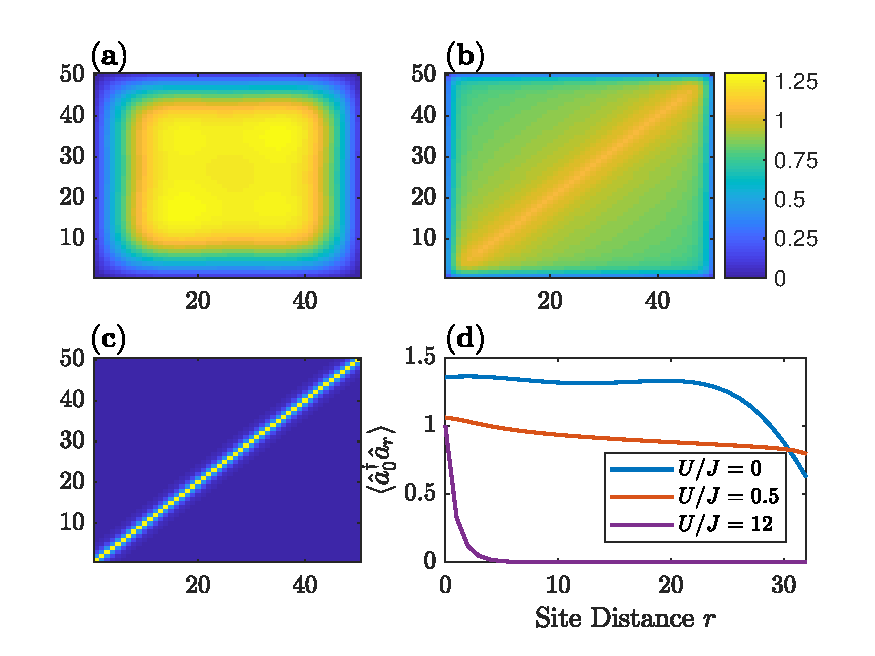
\includegraphics[width=0.8\textwidth]{Figures/DensityMatrices.pdf}
    \caption{\textit{\textbf{(a-c)} Density matrices of a 50 site system for $U/J = 0, \; 0.5, \; 12$. \textbf{(d)} entries of the 15th row of the density matrices plotted as a function of distance from the diagonal, $r$. }}
    \label{fig:DensityMatrices}
\end{figure}
According to eq. \eqref{eq:corrfunction}, correlation functions are given by a linear combination of exponential functions in the MPS description. Therefore, matrix product states struggle describing long range correlations, such as the superfluid single-particle correlations. While single-particle correlations decay exponentially for the Mott-Insulator, it decays following a power-law for superfluids
\begin{equation}
	\braket{\hat{a}_{i}^{\dag} \hat{a}_{j}} \sim |i - j|^{-K_b /2} \; ,
	\label{eq:superfluidCorrelation}
\end{equation}
where $K_b$ is the Tomonaga-Luttinger parameter \cite{characPhases}. For short distances eq. \eqref{eq:corrfunction} is able to accurately approximate a power-law, however, only the slowest exponential decay will survive as distances grow larger. Hence, the correlation turns into a pure exponential decay with $\xi = -1/ \ln \lambda$, where $\lambda$ is the largest eigenvalue of $\hat{E}$ contributing to the correlation.\\
To demonstrate the correlation properties of matrix product states, consider figure \ref{fig:DensityMatrices} depicting the density matrix with entries $\rho_{i,j} = \bra{\psi} \hat{a}_{i}^{\dag} \hat{a}_{j} \ket{\psi}$ for the ground state of a Bose-Hubbard system with $L = 50$ sites and unit occupancy. The ground state was found at various fractions of $U/J$ using the DMRG algorithm detailed in Section \ref{sec:DMRG}.
Figures \ref{fig:DensityMatrices}(a) and \ref{fig:DensityMatrices}(c) show the density matrix plotted for the superfluid and the Mott-Insulator limit respectively. In the superfluid limit, long-range correlations are present, which is seen by large off-diagonal elements. However, since all correlations decay exponentially in the MPS description, the algorithm has difficulty approximating the very long range correlations of the system. This is visualized in figure \ref{fig:DensityMatrices}(d), where the correlation function is plotted against distance from the diagonal. The superfluid graph has a hump on it, which is an artifact of the MPS description and DMRG algorithm. Due to the very long correlation length, the graph should be almost flat except for the rapid drop in the end, which is due to the closed boundary conditions.\\
In the Mott-Insulator limit no interaction takes place between sites, and the correlation length is zero. Hence, the correlation matrix contains only diagonal elements of equal magnitude. Figure \ref{fig:DensityMatrices}(c) shows some off-diagonal elements of non-zero magnitude, since the system is not a pure Mott-Insulator at $U/J = 12$. Nevertheless, the correlations are well described by only a single exponential function, as seen by the figure.\\
Finally, figure \ref{fig:DensityMatrices}(b) illustrates the density matrix for a system with $U/J = 0.5$, which is primarily a superfluid. The particles are not completely de-localized, which is noticeable from the well defined diagonal. Plotting the correlation function reveals the best approximation being a power-law, confirming the system is indeed a superfluid. 
